\section{Appendix}
\label{sec:implementation_details}

\subsection{Model Architecture Details}
\label{subsec:model_hyperparams}


% \subsection{Scaling}
% \label{subsec:scaling}
We develop $5$ Chinese CLIP models of different sizes, spanning from around $77$ to $958$ million parameters. 
We include $1$ ResNet-50 model $\text{CN-CLIP}\rm_{RN50}$ and $4$ ViT models, i.e., $\text{CN-CLIP}\rm_{ViT\text{-}B/16}$, $\text{CN-CLIP}\rm_{ViT\text{-}L/14}$, $\text{CN-CLIP}\rm_{ViT\text{-}L/14@336px}$ and $\text{CN-CLIP}\rm_{ViT\text{-}H/14}$, where models are pretrained on images of the resolution of $224 \times 224$ without specification. 
Table~\ref{tb:modelcard} presents the details of the model architecture. 
The smallest model $\text{CN-CLIP}\rm_{RN50}$ consists of a ResNet-50 for the image encoder and a RBT3 for the text encoder. 
The base-size model $\text{CN-CLIP}\rm_{ViT\text{-}B/16}$ consists of a ViT-B/16@224px for the image encoder and a RoBERTa-wwm-Base for the text encoder. 
The large-size model $\text{CN-CLIP}\rm_{ViT\text{-}L/14}$ consists of a ViT-L/14@224px for the image encoder and a RoBERTa-wwm-Base for the text encoder, while $\text{CN-CLIP}\rm_{ViT\text{-}L/14@336px}$ consists of a ViT-L/14@336px and a RoBERTa-wwm-Base. 
Specifically, we pretrain $\text{CN-CLIP}\rm_{ViT\text{-}L/14@336px}$ by continuing pretraining on the pretrained $\text{CN-CLIP}\rm_{ViT\text{-}L/14}$. 
For the adaptation to a larger resolution, we initialize the image positional embedding by applying interpolation to the positional embedding of $\text{CN-CLIP}\rm_{ViT\text{-}L/14}$, following \citet{openclip}. 
The huge-size model $\text{CN-CLIP}\rm_{ViT\text{-}H/14}$ consists of a ViT-H/14 for the image encoder and RoBERTa-wwm-Large for the text encoder. 
More implementation details are presented in Appendix~\ref{sec:implementation_details}.

\begin{table*}[t]
\center
\small
\vskip 0.15in
\begin{adjustbox}{max width=1.\textwidth}
\begin{tabular}{@{\extracolsep{\fill}}lcccccc}
\toprule
  Model
  & \#Params (All)
  & Backbone (I)
  & \#Params (I)
  & Backbone (T)
  & \#Params (T)
  & Resolution
  \\
\midrule
    $\text{CN-CLIP}\rm_{RN50}$
    & 77M & ResNet-50 & 38M & RBT3 & 39M & $224\times224$
    \\
    $\text{CN-CLIP}\rm_{ViT\text{-}B/16}$
    & 188M & ViT-B/16 & 86M & RoBERTa-wwm-Base & 102M & $224\times224$
    \\
    $\text{CN-CLIP}\rm_{ViT\text{-}L/14}$
    & 406M & ViT-L/14 & 304M & RoBERTa-wwm-Base & 102M & $224\times224$
    \\
    $\text{CN-CLIP}\rm_{ViT\text{-}L/14@336px}$
    & 407M & ViT-L/14 & 304M & RoBERTa-wwm-Base & 102M & $336\times336$
    \\
    $\text{CN-CLIP}\rm_{ViT\text{-}H/14}$
    & 958M & ViT-H/14 & 632M & RoBERTa-wwm-Large & 326M & $224\times224$
    \\
\bottomrule
\end{tabular}
\end{adjustbox}
\caption{Hyperparameters of Chinese CLIP models of different sizes. }
\label{tb:modelcard}
\end{table*}

\begin{table*}[t]
\center
\small
% \vskip 0.15in
% \begin{adjustbox}{max width=1.\textwidth}
\begin{tabular}{@{\extracolsep{\fill}}lccccccc}
\toprule
  \multirow{2}{*}{Model}
  & Embedding
  & \multicolumn{3}{c}{Vision Transformer}
  & \multicolumn{3}{c}{Text Transformer}
  \\
  & dimension
  & layers
  & width
  & heads
  & layers
  & width
  & heads
  \\
\midrule
    % $\text{CN-CLIP}\rm_{RN50}$
    % & 77M 
    % & ResNet-50 
    % & 38M 
    % & RBT3 
    % & 39M 
    % & $224\times224$
    % \\
    $\text{CN-CLIP}\rm_{ViT\text{-}B/16}$
    & 512
    & 12
    & 768
    & 12
    & 12
    & 768
    & 12
    \\
    $\text{CN-CLIP}\rm_{ViT\text{-}L/14}$
    & 768
    & 24
    & 1,024
    & 16
    & 12
    & 768
    & 12
    \\
    $\text{CN-CLIP}\rm_{ViT\text{-}L/14@336px}$
    & 768
    & 24
    & 1,024
    & 16
    & 12
    & 768
    & 12
    \\
    $\text{CN-CLIP}\rm_{ViT\text{-}H/14}$
    & 1,024
    & 32
    & 1,280
    & 16
    & 24
    & 1,024
    & 24
    \\
\bottomrule
\end{tabular}
% \end{adjustbox}
\caption{Detailed architecture hyperparameters of ViT-based CN-CLIP models.}
\label{tb:detailed_architecture_vit}
\end{table*}

\begin{table*}[t]
\center
\small
% \vskip 0.15in
% \begin{adjustbox}{max width=1.\textwidth}
\begin{tabular}{@{\extracolsep{\fill}}lcccccc}
\toprule
  \multirow{2}{*}{Model}
  & Embedding
  & \multicolumn{2}{c}{ResNet}
  & \multicolumn{3}{c}{Text Transformer}
  \\
  & dimension
  & blocks
  & width
  & layers
  & width
  & heads
  \\
\midrule
    $\text{CN-CLIP}\rm_{RN50}$
    & 1,024
    & (3, 4, 6, 3)
    & 2,048
    & 3
    & 768
    & 12
    \\
\bottomrule
\end{tabular}
% \end{adjustbox}
\caption{Detailed architecture hyperparameters of ResNet-based $\text{CN-CLIP}\rm_{RN50}$.}
\label{tb:detailed_architecture_rn}
\end{table*}
% As mentioned in Section~\ref{subsec:scaling} and Table~\ref{tb:modelcard}, we release $5$ Chinese CLIP models of different sizes. 
We provide more details of their model architectures in Table~\ref{tb:detailed_architecture_vit} and Table~\ref{tb:detailed_architecture_rn}. We keep the architecture of ResNet-50, ViT-B/16, and ViT-L/14 backbones conformed with OpenAI CLIP and the architecture of ViT-H/14 same with LAION CLIP\footnote{\url{https://laion.ai/blog/large-openclip/}}. 
This enables us to initialize the Chinese CLIP image encoders with their weights. 
The text encoders are Chinese Roberta models~\cite{wwm}. Specifically, our most lightweight tiny-size Chinese CLIP uses the architecture of the $3$-layer RBT3 model. The base-size and large-size Chinese CLIP models use the $12$-layer architecture of RoBERTa-wwm-Base. For the huge-size CN-CLIP, we use the $24$-layer architecture of RoBERTa-wwm-Large. The vocabulary size of text tokenizer is $21,128$.

\subsection{Pretraining Details}
\label{subsec:pretraining_details}

\paragraph{Initialization} As mentioned in Section~\ref{subsec:pretraining_method}, we initialize the image encoders of $\text{CN-CLIP}\rm_{RN50}$, $\text{CN-CLIP}\rm_{ViT\text{-}B/16}$ and $\text{CN-CLIP}\rm_{ViT\text{-}L/14}$ using the OpenAI CLIP weights. The image encoder of $\text{CN-CLIP}\rm_{ViT\text{-}H/14}$ is initialized with LAION CLIP. 
Besides the ResNet or ViT parameters, the temperature and visual output projection parameters are also initialized with the pretrained CLIP weights. 
For the text encoder, we initialize the parameters using the released Chinese Roberta weights of the corresponding model scale, with their pooler weights discarded. The text output projection weight is randomly initialized with normal distribution.

\begin{table}[t]
\center
\small
\begin{tabular}{lc}
\toprule
  Hyperparameters
  & Value
  \\
\midrule
    Batch size
    & $32,768$
    \\
    Maximum text length
    & $50$
    \\             
    Peak learning rate
    & $1e-4$
    \\
    Learning rate schedule
    & Cosine
    \\    
    % Training epochs
    % & $20$
    % & $44$
    % & $64$
    % & $26$
    % \\
    Maximum temperature
    & $100$
    \\
    Weight decay
    & $1e-3$
    \\        
    Warmup iterations
    & $5,000$
    \\        
    Adam $\beta_1$
    & $0.9$
    \\      
    Adam $\beta_2$
    & $0.999$ (ResNet), $0.98$ (ViT)
    \\     
    Adam $\epsilon$
    & $1e-8$ (ResNet), $1e-6$ (ViT)
    \\        
\bottomrule
\end{tabular}
\caption{Common pretraining hyperparameters in the first stage.}
\label{tb:hyperparams_stage1}
\end{table}

\paragraph{Stage 1} 
The pretraining hyperparameters of Stage 1 are shown in Table~\ref{tb:hyperparams_stage1}, which are shared for $\text{CN-CLIP}\rm_{RN50}$, $\text{CN-CLIP}\rm_{ViT\text{-}B/16}$, $\text{CN-CLIP}\rm_{ViT\text{-}L/14}$ and $\text{CN-CLIP}\rm_{ViT\text{-}H/14}$. 
The values of hyperparameters are generally similar to those in OpenAI CLIP~\citep{clip}. 
As to data augmentation, we use random resize cropping and AutoAugment~\citep{autoaugment} on input images. We leverage all-gather communications across GPU workers to compute contrastive loss on the global batch. The above $4$ models are pretrained for around $20$, $44$, $64$, and $26$ epochs in this stage respectively, with the image encoder frozen. The running variance and mean of batch normalization layers are not updated in this stage for $\text{CN-CLIP}\rm_{RN50}$. The optimal epochs of pretraining are determined by measuring the mean-recall under the $3$ downstream zero-shot retrieval tasks during training. Mixed-precision training is activated. 
In this stage, we pretrain $1.6$ days using $64$ NVIDIA V100 GPUs for $\text{CN-CLIP}\rm_{RN50}$, $4.5$ days using $128$ NVIDIA V100 GPUs for $\text{CN-CLIP}\rm_{ViT\text{-}B/16}$, $11.5$ days using $128$ NVIDIA V100 GPUs for $\text{CN-CLIP}\rm_{ViT\text{-}L/14}$ and $3.8$ days using $184$ NVIDIA A100 GPUs for $\text{CN-CLIP}\rm_{ViT\text{-}H/14}$.

\paragraph{Stage 2} 
In Stage 2, we unfreeze the image encoder and update all the model parameters. Except for the peak learning rate, batch size and training epochs, all other hyperparameters mentioned in Stage 1 are kept unchanged. We decrease the learning rate to $2e-5$ for subtler optimization. % Updating all the parameters will cost more GPU memory during backward computation. 
For $\text{CN-CLIP}\rm_{RN50}$, $\text{CN-CLIP}\rm_{ViT\text{-}B/16}$ and $\text{CN-CLIP}\rm_{ViT\text{-}L/14}$, the batch size is shrunk to $16,384$, $16,384$ and $4,608$ respectively due to the limitation in GPU memory. When scaling to $\text{CN-CLIP}\rm_{ViT\text{-}H/14}$, we implement gradient checkpointing, which enables a larger batch size of $32,768$. These $4$ models are pretrained for around $44$, $15$, $7$ and $7$ epochs in Stage 2, respectively.
In this stage, we pretrain $\text{CN-CLIP}\rm_{RN50}$ for $5.8$ days using $64$ NVIDIA V100 GPUs, $\text{CN-CLIP}\rm_{ViT\text{-}B/16}$ for $3.0$ days using $128$ NVIDIA V100 GPUs, $\text{CN-CLIP}\rm_{ViT\text{-}L/14}$ for $8.0$ days using $128$ Nvidia V100 GPUs, and $\text{CN-CLIP}\rm_{ViT\text{-}H/14}$ for $2.2$ days using $184$ NVIDIA A100 GPUs. 

To pretrain a model of a larger resolution, we implement interpolation to the image positional embedding of $\text{CN-CLIP}\rm_{ViT\text{-}L/14}$ for adapting to a larger resolution and continue pretraining with images of the resolution of $336 \times 336$. 
We start from $\text{CN-CLIP}\rm_{ViT\text{-}L/14}$ and continue pretraining by $2$ epochs. 
The pretraining only costs the use of $128$ NVIDIA A100 GPUs for $0.7$ days.

\subsection{Finetuning Details}
% % This must be in the first 5 lines to tell arXiv to use pdfLaTeX, which is strongly recommended.
% \pdfoutput=1
% % In particular, the hyperref package requires pdfLaTeX in order to break URLs across lines.

% \documentclass[11pt]{article}

% % Remove the "review" option to generate the final version.
% \usepackage[review]{acl}

% % Standard package includes
% \usepackage{times}
% \usepackage{latexsym}

% % For proper rendering and hyphenation of words containing Latin characters (including in bib files)
% \usepackage[T1]{fontenc}
% % For Vietnamese characters
% % \usepackage[T5]{fontenc}
% % See https://www.latex-project.org/help/documentation/encguide.pdf for other character sets

% % This assumes your files are encoded as UTF8
% \usepackage[utf8]{inputenc}

% This is not strictly necessary, and may be commented out,
% but it will improve the layout of the manuscript,
% and will typically save some space.
% \usepackage{microtype}
% \usepackage{graphicx}
% \usepackage{subfigure}
% \usepackage{booktabs} % for professional tables

% \usepackage{amsfonts}
% \usepackage{stfloats}
% \usepackage{ulem}

% \usepackage{amsmath}
% % Attempt to make hyperref and algorithmic work together better:
% \newcommand{\theHalgorithm}{\arabic{algorithm}}
% \newcommand{\tabincell}[2]{\begin{tabular}{@{}#1@{}}#2\end{tabular}}
% \usepackage{adjustbox}
% \usepackage{multirow}
% \usepackage{array}
% \usepackage{float}
% \usepackage{caption}
% \usepackage{balance}
% \usepackage{flushend}
% \usepackage{color}

% \definecolor{light-gray}{gray}{0.5}
% % If the title and author information does not fit in the area allocated, uncomment the following
% %
% %\setlength\titlebox{<dim>}
% %
% % and set <dim> to something 5cm or larger.

% \title{Chinese CLIP: Contrastive Vision-Language Pretraining in Chinese}
% \begin{document}


\begin{table*}[t]
\center
% \small
% \vskip 0.15in
\begin{adjustbox}{max width=1.\textwidth}
\begin{tabular}{@{\extracolsep{\fill}}lccccccccccccc}
\toprule
  \multirow{2}{*}{Model}
  & \multicolumn{3}{c}{Batch size}
  & \multicolumn{3}{c}{Peak learning rate}
  & \multicolumn{3}{c}{Maximum epochs}
  & \multicolumn{3}{c}{Warmup iterations}

  \\
  & MUGE
  & Flickr
  & COCO
  & MUGE
  & Flickr
  & COCO
  & MUGE
  & Flickr
  & COCO
  & MUGE
  & Flickr
  & COCO
  \\
\midrule
    $\text{CN-CLIP}\rm_{RN50}$
    & 24,576
    & 24,576
    & 24,576
    & 5e-5
    & 6e-5
    & 5e-5
    & 60
    & 30
    & 40
    & 100
    & 20
    & 6
    \\
    $\text{CN-CLIP}\rm_{ViT\text{-}B/16}$
    & 12,800
    & 7,680
    & 12,800
    & 2e-5
    & 5e-5
    & 5e-5
    & 20
    & 16
    & 30
    & 40
    & 20
    & 6
    \\
    $\text{CN-CLIP}\rm_{ViT\text{-}L/14}$
    & 4,096
    & 4,096
    & 4,096
    & 3e-5
    & 2e-5
    & 6e-5
    & 20
    & 16
    & 18
    & 100
    & 60
    & 9
    \\
    $\text{CN-CLIP}\rm_{ViT\text{-}L/14@336px}$
    & 8,192
    & 8,192
    & 8,192
    & 2e-5
    & 2e-5
    & 4e-5
    & 20
    & 18
    & 18
    & 100
    & 20
    & 2
    \\
    $\text{CN-CLIP}\rm_{ViT\text{-}H/14}$
    & 20,480
    & 4,096
    & 5,120
    & 2e-5
    & 6e-6
    & 2e-5
    & 20
    & 18
    & 18
    & 20
    & 6
    & 10
    \\
\bottomrule
\end{tabular}
\end{adjustbox}
\caption{Detailed finetuning hyperparameters of CN-CLIP models.}
\label{tb:detailed_finetune}
\end{table*}

% \end{document}
\begin{table*}[t]
\center
\small
% \vskip 0.15in
\begin{adjustbox}{max width=1.\textwidth}
\begin{tabular}{@{\extracolsep{\fill}}lcccccccc}
\toprule
  Tasks
  &\multicolumn{3}{c}{Text-to-Image}
  &\multicolumn{3}{c}{Image-to-Text}
  & 
  \\
% \midrule
  % Setups
  % &\multicolumn{6}{c}{Finetuning}
  % &\multicolumn{4}{c}{Finetuning}
  % \\
\midrule
  Metrics & R@1 & R@5 & R@10 & R@1 & R@5 & R@10 & MR
  \\
\midrule
  $\text{R2D2}\rm_{ViT\text{-}B}$
  & 42.2    & 69.4  & 77.8	& 43.4	& 69.8	& 78.4 & 63.5
  \\
  $\text{R2D2}\rm_{ViT\text{-}L/14}$
  & 60.7    & 82.0  & 86.9  & 61.5  & 82.9  & 87.7  & 77.0
  \\
  $\text{CN-CLIP}\rm_{ViT\text{-}B/16}$
  & 55.4    & 79.0  & 85.2  & 56.6  & 79.5  & 85.6  & 73.5
  \\
  $\text{CN-CLIP}\rm_{ViT\text{-}L/14}$
  & \textbf{61.6}    & \textbf{83.6}  & \textbf{89.0}  & \textbf{62.5}  & \textbf{83.9}  & \textbf{89.1}  & \textbf{78.3}
  \\

\bottomrule
\end{tabular}
\end{adjustbox}
\caption{Finetuning results on ICR dataset. We report the performance of baselines, $\text{CN-CLIP}\rm_{ViT\text{-}B/16}$ and $\text{CN-CLIP}\rm_{ViT\text{-}L/14}$ on text-to-image and image-to-text retrieval. }
\label{tb:ICR}
\end{table*}
As reported in Table~\ref{tb:muge}, \ref{tb:flickr} and \ref{tb:coco}, we mainly finetune CN-CLIP on $3$ cross-modal retrieval datasets: MUGE, Flickr30K-CN, and COCO-CN.
Most finetuning experiments are conducted on $32$ NVIDIA A100 GPUs.
The finetuning strategy and loss are consistent with the pretraining process.
For time efficiency and full utilization of computation resources, we set the batch size as large as possible.
We implement gradient checkpointing in the finetuning process of $\text{CN-CLIP}\rm_{ViT\text{-}L/14@336px}$ and $\text{CN-CLIP}\rm_{ViT\text{-}H/14}$ for a larger batch size.
Table~\ref{tb:detailed_finetune} shows the specific settings of batch size, peaking learning rate, maximum epochs, and warmup iterations in the finetuning process.
We set other hyperparameters to be the same as those in pretraining by default.
We save the model parameters at the end of each epoch.
For MUGE, we report the best results on the validation set.
For Flickr30K-CN and COCO-CN, we choose the checkpoint with the best performance on the validation set and report the results on the test set.
% In particular, we find that under the same setting of batch size, a larger peak learning rate will lead to , but usually will also reach a higher MR. A relatively small peak learning rate will delay the occurrence of over fitting, but the maximum MR can be lower.


\subsection{Cross-modal Retrieval with Longer Texts}
The results reported in Section~\ref{subsubsec:results} demonstrate the excellent cross-modal retrieval capability of Chinese CLIP.
Note that the average text lengths of MUGE, Flickr30K-CN, and COCO-CN are $7.4$, $19.7$, and $16.8$, respectively.
We also conduct finetuning experiments on the ICR~\citep{r2d2} dataset with an average text length of $45.3$. 
Experimental results are shown in Table~\ref{tb:ICR}.
Since the texts in the ICR dataset are longer, we set the maximum text length to $128$ for finetuning.
The results show that Chinese CLIP achieves state-of-the-art performance in cross-modal retrieval tasks with longer texts.

% We also conducted finetuning experiments on ICR~\citep{r2d2} dataset for $\text{CN-CLIP}\rm_{ViT\text{-}B/16}$ and $\text{CN-CLIP}\rm_{ViT\text{-}L/14}$. Since the text in the ICR dataset is longer, we set the maximum text length to $128$ when finetuning. $\text{CN-CLIP}\rm_{ViT\text{-}B/16}$ and $\text{CN-CLIP}\rm_{ViT\text{-}L/14}$ achieve $73.5$ and $78.3$ 


\subsection{Details About Experiments on Zero-shot Image Classification}

\begin{table*}[t]
\center
\small
\vskip 0.15in
\begin{adjustbox}{max width=1.\textwidth}
\begin{tabular}{@{\extracolsep{\fill}}lccc}
\toprule
%   Dataset & Metric & $\text{CLIP}\rm_{ViT\text{-}B/32}$ & $\text{CLIP}\rm_{ViT\text{-}B/16}$ & $\text{CLIP}\rm_{ViT\text{-}L/14}$ 
%   & $\text{CN-CLIP}\rm_{RN50}$ & $\text{CN-CLIP}\rm_{ViT\text{-}B/16}$ & $\text{CN-CLIP}\rm_{ViT\text{-}L/14}$ 
%   & $\text{CN-CLIP}\rm_{ViT\text{-}L/14@336px}$ & $\text{CN-CLIP}\rm_{ViT\text{-}H/14}$ 
%   \\
Dataset & \#Labels & Test Size & Metric \\
\midrule
  Caltech-101~\citep{caltech} & 101 & 6,084 & Mean-per-class  \\
  CIFAR-10~\citep{cifar} & 10 & 10,000 &  Accuracy   \\
  CIFAR-100~\citep{cifar} & 100 & 10,000 & Accuracy   \\
  Country-211~\citep{clip} & 211 & 21,100 & Accuracy   \\
  DTD~\citep{dtd} & 47 & 1,880 & Accuracy  \\
  EuroSAT~\citep{eurosat} & 10 & 5,000 & Accuracy  \\
  FER-2013~\citep{clip} & 7 & 3,589 & Accuracy  \\
  FGVC-Aircraft~\citep{fgvc} & 100 & 3,333 & Mean-per-class \\
  Food-101~\citep{food101} & 101 & 25,250 & Accuracy \\
  GTSRB~\citep{gtsrb} & 43 & 12,630 & Accuracy  \\
  Hateful-Memes~\citep{hateful} & 2  & 500 & ROC AUC \\
  KITTI-Distance~\citep{kitti} & 4 & 711 & Accuracy  \\
  MNIST~\citep{mnist} & 10 & 10,000 & Accuracy \\
  Oxford Flowers-102~\citep{flowers} & 102 & 6,149 & Mean-per-class  \\
  Oxford-IIIT Pets~\cite{pets} & 37 & 3,669 & Mean-per-class \\
  PatchCamelyon~\citep{patchcamelyon} & 2 & 32,768 & Accuracy  \\
  Rendered-SST2~\citep{clip} & 2 & 1,821 & Accuracy  \\
  RESISC-45~\citep{resisc45} & 45 & 25,200 & Accuracy \\
  Stanford-Cars~\citep{stanford_cars} & 196 & 8,041 & Accuracy  \\
  Pascal VOC-2007~\citep{voc} & 20 & 4,952 & 11-point mAP \\
\bottomrule
\end{tabular}
\end{adjustbox}
\caption{Details of the image classification datasets in the ELEVATER benchmark. }
\label{tb:icinw}
\end{table*}

\begin{table*}[t]
\center
\small
\vskip 0.15in
\begin{adjustbox}{max width=1.\textwidth}
\begin{tabular}{@{\extracolsep{\fill}}lccccc}
\toprule
%   Dataset & Metric & $\text{CLIP}\rm_{ViT\text{-}B/32}$ & $\text{CLIP}\rm_{ViT\text{-}B/16}$ & $\text{CLIP}\rm_{ViT\text{-}L/14}$ 
%   & $\text{CN-CLIP}\rm_{RN50}$ & $\text{CN-CLIP}\rm_{ViT\text{-}B/16}$ & $\text{CN-CLIP}\rm_{ViT\text{-}L/14}$ 
%   & $\text{CN-CLIP}\rm_{ViT\text{-}L/14@336px}$ & $\text{CN-CLIP}\rm_{ViT\text{-}H/14}$ 
%   \\
\multirow{2}{*}{Dataset} & CN-CLIP & CN-CLIP & CN-CLIP & CN-CLIP & CN-CLIP \\
 & $\rm_{RN50}$ & $\rm_{ViT\text{-}B/16}$ & $\rm_{ViT\text{-}L/14}$ & $\rm_{ViT\text{-}L/14@336px}$ & $\rm_{ViT\text{-}H/14}$ \\
\midrule
  Caltech-101  & 77.3 & 84.9 & 88.5 & 88.8 & 90.6  \\
  CIFAR-10  & 72.7 & 92.0 & 94.9 & 94.1 & 96.0  \\
  CIFAR-100   & 40.6 & 64.4 & 75.1 & 73.5 & 79.7  \\
  Country-211   & 7.7 & 15.2 & 21.0 & 25.4 & 25.3  \\
  DTD   & 36.9 & 43.6 & 44.2 & 43.8 & 51.2  \\
  EuroSAT   & 27.0 & 46.9 & 56.9 & 50.7 & 52.0  \\
  FER-2013   & 21.9 & 47.2 & 54.6 & 55.1 & 49.2  \\
  FGVC-Aircraft  & 5.4 & 12.8 & 16.0 & 17.1 & 26.2  \\
  Food-101   & 39.8 & 62.4 & 69.4 & 73.9 & 74.6  \\
  GTSRB   & 22.3 & 28.4 & 37.3 & 35.5 & 38.5  \\
  Hateful-Memes   & 50.3 & 56.2 & 53.4 & 52.8 & 54.7  \\
  KITTI-Distance  & 30.2 & 33.5 & 49.9 & 49.8 & 39.1  \\
  MNIST   & 50.2 & 67.6 &69.8 & 65.0 & 79.4  \\
  Oxford Flowers-102   & 30.7 & 52.2 &62.5 & 64.8 & 68.4  \\
  Oxford-IIIT Pets   & 48.7 & 73.0 &81.6 & 83.1 & 83.5  \\
  PatchCamelyon  & 47.7 & 54.0 & 63.5 & 62.9 & 52.4  \\
  Rendered-SST2  & 50.1 & 52.3 & 61.4 & 62.9 & 61.0  \\
  RESISC-45   & 49.3 & 58.7 & 65.2 & 65.8 & 66.9  \\
  Stanford-Cars  & 27.3 & 42.3 &49.8 & 54.1 & 71.8  \\
  VOC-2007  & 82.1 & 83.3 & 84.5 & 84.9 & 84.9  \\
  Average  & 40.9 & 53.5 & 60.0 & 60.2 & 62.3  \\
\bottomrule
\end{tabular}
\end{adjustbox}
\caption{Experimental results of the zero-shot image classification performance of models on ICinW. }
\label{tb:zs}
\end{table*}

% \begin{table*}[t]
% \center
% \small
% \vskip 0.15in
% \begin{adjustbox}{max width=1.\textwidth}
% \begin{tabular}{@{\extracolsep{\fill}}lcccccccc}
% \toprule
% %   Dataset & Metric & $\text{CLIP}\rm_{ViT\text{-}B/32}$ & $\text{CLIP}\rm_{ViT\text{-}B/16}$ & $\text{CLIP}\rm_{ViT\text{-}L/14}$ 
% %   & $\text{CN-CLIP}\rm_{RN50}$ & $\text{CN-CLIP}\rm_{ViT\text{-}B/16}$ & $\text{CN-CLIP}\rm_{ViT\text{-}L/14}$ 
% %   & $\text{CN-CLIP}\rm_{ViT\text{-}L/14@336px}$ & $\text{CN-CLIP}\rm_{ViT\text{-}H/14}$ 
% %   \\
% \multirow{2}{*}{Dataset} & CLIP & CLIP & CLIP & CN-CLIP & CN-CLIP & CN-CLIP & CN-CLIP & CN-CLIP \\
%  & $\rm_{ViT\text{-}B/32}$ & $\rm_{ViT\text{-}B/16}$ & $\rm_{ViT\text{-}L/14@336px}$ & $\rm_{RN50}$ & $\rm_{ViT\text{-}B/16}$ & $\rm_{ViT\text{-}L/14}$ & $\rm_{ViT\text{-}L/14@336px}$ & $\rm_{ViT\text{-}H/14}$ \\
% \midrule
%   Caltech-101 & 87.5 & 88.9 & \textbf{92.4} & 77.3 & 84.9 & 88.5 & 88.8 & 90.6  \\
%   CIFAR-10  & 89.9 & 90.8 & 94.9 & 72.7 & 92.0 & 94.9 & 94.1 & \textbf{96.0}  \\
%   CIFAR-100  & 65.1 & 68.2 & 77.0 & 40.6 & 64.4 & 75.1 & 73.5 & \textbf{79.7}  \\
%   Country-211  & 17.2 & 22.8 & \textbf{34.5} & 7.7 & 15.2 & 21.0 & 25.4 & 25.3  \\
%   DTD  & 44.4 & 44.7 & \textbf{56.0} & 36.9 & 43.6 & 44.2 & 43.8 & 51.2  \\
%   EuroSAT  & 45.6 & 54.7 & \textbf{63.0} & 27.0 & 46.9 & 56.9 & 50.7 & 52.0  \\
%   FER-2013  & 42.1 & 48.5 & 48.3 & 21.9 & 47.2 & 54.6 &\textbf{ 55.1} & 49.2  \\
%   FGVC-Aircraft  & 19.6 & 24.3 & \textbf{33.3} & 5.4 & 12.8 & 16.0 & 17.1 & 26.2  \\
%   Food-101  & 84.0 & 88.7 & \textbf{93.9} & 39.8 & 62.4 & 69.4 & 73.9 & 74.6  \\
%   GTSRB  & 32.8 & 43.6 & \textbf{52.3} & 22.3 & 28.4 & 37.3 & 35.5 & 38.5  \\
%   Hateful-Memes  & 56.0 & 58.1 & \textbf{60.0} & 50.3 & 56.2 & 53.4 & 52.8 & 54.7  \\
%   KITTI-Distance  & 29.0 & 26.7 & 11.5 & 30.2 & 33.5 & 49.9 & \textbf{49.8} & 39.1  \\
%   MNIST  & 48.1 & 52.1 & 79.0 & 50.2 & 67.6 &69.8 & 65.0 & \textbf{79.4}  \\
%   Oxford Flowers-102  & 66.5 & 69.4 & \textbf{78.5} & 30.7 & 52.2 &62.5 & 64.8 & 68.4  \\
%   Oxford-IIIT Pets  & 87.1 & 89.0 & \textbf{93.8} & 48.7 & 73.0 &81.6 & 83.1 & 83.5  \\
%   PatchCamelyon  & 60.7 & 54.0 & 62.3 & 47.7 & 54.0 &\textbf{63.5} & 62.9 & 52.4  \\
%   Rendered-SST2  & 58.4 & 60.6 & \textbf{70.6} & 50.1 & 52.3 & 61.4 & 62.9 & 61.0  \\
%   RESISC-45  & 60.0 & 65.6 & \textbf{71.4} & 49.3 & 58.7 & 65.2 & 65.8 & 66.9  \\
%   Stanford-Cars  & 59.7 & 64.8 & \textbf{79.3} & 27.3 & 42.3 &49.8 & 54.1 & 71.8  \\
%   VOC-2007  & 82.6 & 83.7 & 84.0 & 82.1 & 83.3 & 84.5 & \textbf{84.9} & \textbf{84.9}  \\
%   Average & 56.8 & 60.0 & \textbf{66.8} & 40.9 & 53.5 & 60.0 & 60.2 & 62.3  \\
% \bottomrule
% \end{tabular}
% \end{adjustbox}
% \caption{Experimental results of the zero-shot image classification performance of models on ICinW. }
% \label{tb:zs}
% \end{table*}

We present the data statistics and metrics of the $20$ image classification datasets of the track ICinW in the ELEVATER benchmark in Table~\ref{tb:icinw}. 
For the adaptation of Chinese CLIP to the English-native benchmark, we apply a series of preprocessing strategies. Specifically, we translate the text descriptions of the labels and the templates for manual prompts to Chinese. 
For example, the labels in CIFAR-10 include ``car, dog, ...'', and we manually translate the words into Chinese. 
There are also particular cases, such as the labels in FGVC-Aircraft~\citep{fgvc}, which are difficult to translate or transliterate. 
We search the names on Google and figure out the best Chinese name for each label. 
Be that as it may, we cannot guarantee that we have the best Chinese translation, and more importantly, it is still hard for the Chinese pretrained model to understand some of the concepts, which may lead to unsatisfactory performance in the related downstream tasks. 
As to the templates, for some datasets, we use our translation of the templates provided by the ELEVATER toolkit,\footnote{\url{https://github.com/Computer-Vision-in-the-Wild/Elevater\_Toolkit\_IC}} and for the others, we use the translation of the templates from OpenAI CLIP.

We present the experimental results of all Chinese CLIP models on zero-shot image classification in Table~\ref{tb:zs}. 
It can be found that the scaling of model size can consistently bring improvements in model performance. 
The predictable improvements of scaling Chinese CLIP indicate that we can further scale up the model for better performance in the future work.  
However, it is still a pity that the tiny-size $\text{CN-CLIP}\rm_{RN50}$ saliently performs much worse than the ViT variants which are significantly larger. 
This shows that there is still much room for the small model to improve, and the knowledge transfer of CLIP from large models to small models should be an important research topic in multimodal representation learning. 

\subsection{Deployment}
\label{appendix:deployment}

Chinese CLIP is supported to be deployed into ONNX-based\footnote{\url{https://onnx.ai/}} and TensorRT-based\footnote{\url{https://developer.nvidia.com/tensorrt}} models, enabling faster text and vision representation generation (especially for online inference). In this section, we provide more details on the model conversion, as well as the performance improvement. 
% The code for ONNX-based and TensorRT-based model deployment is opensourced.

Specifically, we employ the ONNX module in PyTorch with \textsc{onnxmltools}\footnote{\url{https://github.com/onnx/onnxmltools}} package to convert Chinese CLIP PyTorch models to ONNX-based models in FP16 precision. With the support of \textsc{onnxruntime-gpu}\footnote{\url{https://onnxruntime.ai/docs/install}} package, the ONNX-based models are able to infer on NVIDIA GPUs. The \textsc{TensorRT} package enables the TensorRT-based models obtained from ONNX-based models and provides the GPU inference runtime. Our TensorRT-based models are also in FP16 precision.

We benchmark the PyTorch implemented Chinese CLIP models with converted ONNX-based and TensorRT-based models using a server with a single NVIDIA T4 GPU. The server contains \num{16} Intel Xeon (Skylake) Platinum 8163 CPU cores with \num{64}GB memory. For each model, we inference the vision and text representations for $100$ batches and compute the average time. Simulating the scenario of online deployment, we use batch size of $1$. All the models infer with FP16 precision. Table~\ref{tb:deployment_speed} shows the comparisons of inference time cost. For almost all the model scales, ONNX-based and TensorRT-based models have optimized inference speed over native PyTorch implemented Chinese CLIP models, especially on smaller model sizes. For vision representation inference, the TensorRT-based models are around $1.3$ ($\text{CN-CLIP}\rm_{ViT\text{-}H/14}$) to $9.5$ ($\text{CN-CLIP}\rm_{RN50}$) times as fast as the Pytorch-based models. For text representation inference, the TensorRT-based models are around $6.2$ ($\text{CN-CLIP}\rm_{ViT\text{-}H/14}$) to $8.2$ ($\text{CN-CLIP}\rm_{ViT\text{-}L/14}$) times as fast as the PyTorch counterparts.

\begin{table*}[t]
\center
\small
% \vskip 0.15in
\begin{adjustbox}{max width=1.\textwidth}
\begin{tabular}{@{\extracolsep{\fill}}lccccccc}
\toprule
  Inference Time per Sample (ms)
  &\multicolumn{3}{c}{Vision Representation}
  &\multicolumn{3}{c}{Text Representation}
  \\
\midrule
  Model Scale & PyTorch & ONNX & TensorRT & PyTorch & ONNX & TensorRT
  \\
\midrule
  $\text{CN-CLIP}\rm_{RN50}$
  & 12.93	& 5.04	& \textbf{1.36} & 	3.64 & 	0.95 &	\textbf{0.58}
  \\
  $\text{CN-CLIP}\rm_{ViT\text{-}B/16}$
  & 11.12	& 4.92	& \textbf{3.58}	& 12.47	& 3.42	& \textbf{1.54}
  \\
  $\text{CN-CLIP}\rm_{ViT\text{-}L/14}$
  & 21.19	& 17.10	& \textbf{13.08}	& 12.45	& 3.48	& \textbf{1.52}
  \\
  $\text{CN-CLIP}\rm_{ViT\text{-}L/14@336px}$
  & 47.11	& 48.40	& \textbf{31.59}	& 12.24	& 3.25	& \textbf{1.54}
  \\
  $\text{CN-CLIP}\rm_{ViT\text{-}H/14}$
  & 35.10	& 34.00	& \textbf{26.98}	& 23.98	& 6.01	& \textbf{3.89}
  \\  

\bottomrule
\end{tabular}
\end{adjustbox}
\caption{Inference speed comparisons among PyTorch, ONNX and TensorRT Chinese CLIP models.}
\label{tb:deployment_speed}
\end{table*}

We also evaluate the quality of ONNX-based and TensorRT-based model representations by measuring their zero-shot performance on MUGE retrieval dataset. Table~\ref{tb:deployment_muge} provides the experimental zero-shot results, which shows that the converted ONNX-based or TensorRT-based models keeps the quality of vision and text representations well, with no more than $0.1$ MR degradation in retrieval performance.

\begin{table*}[t]
\center
\small
% \vskip 0.15in
\begin{adjustbox}{max width=1.\textwidth}
\begin{tabular}{@{\extracolsep{\fill}}lccccc}
\toprule
  \multirow{2}{*}{Model Scale} & \multirow{2}{*}{Framework}
  &\multicolumn{4}{c}{Zero-shot Performance}
  \\
   &  & R@1 & R@5 & R@10 & MR
  \\
\midrule
  \multirow{3}{*}{$\text{CN-CLIP}\rm_{RN50}$}
  & PyTorch	& 42.6	& 68.6	& 77.9	& 63.0 
  \\
  & ONNX	& 43.0 & 68.4 & 78.1 & 63.2
  \\
  & TensorRT	& 42.8 & 68.5 & 78.0 & 63.1
  \\ \midrule
  \multirow{3}{*}{$\text{CN-CLIP}\rm_{ViT\text{-}B/16}$}
  & PyTorch	& 52.1	& 76.7	& 84.4	& 71.1 
  \\
  & ONNX	& 52.0	& 76.8	& 84.3	& 71.1	
  \\
  & TensorRT	& 52.0	& 76.8	& 84.2	& 71.0
  \\ \midrule
  \multirow{3}{*}{$\text{CN-CLIP}\rm_{ViT\text{-}L/14}$}
  & PyTorch	& 56.3	& 79.8	& 86.2	& 74.1 
  \\
  & ONNX	& 56.4	& 80.0	& 86.3	& 74.2	
  \\
  & TensorRT	& 56.3 & 79.9	& 86.5	& 74.2
  \\ \midrule
  \multirow{3}{*}{$\text{CN-CLIP}\rm_{ViT\text{-}L/14@336px}$}
  & PyTorch	& 59.0	& 81.4	& 87.8	& 76.1
  \\
  & ONNX	& 59.2	& 81.4 & 87.6 & 76.1
  \\
  & TensorRT	& 59.2 & 81.7 & 87.5 & 76.1
  \\ \midrule
  \multirow{3}{*}{$\text{CN-CLIP}\rm_{ViT\text{-}H/14}$}
  & PyTorch	& 63.0	& 84.1	& 89.2	& 78.8 
  \\
  & ONNX	& 63.1	& 84.1	& 89.0	& 78.8	
  \\
  & TensorRT	& 63.1	& 84.2	& 89.1	& 78.8
  \\

\bottomrule
\end{tabular}
\end{adjustbox}
\caption{Zero-shot results on MUGE-Retrieval dataset among PyTorch, ONNX and TensorRT Chinese CLIP models.}
\label{tb:deployment_muge}
\end{table*}

\begin{figure*}[h] 
    \centering
    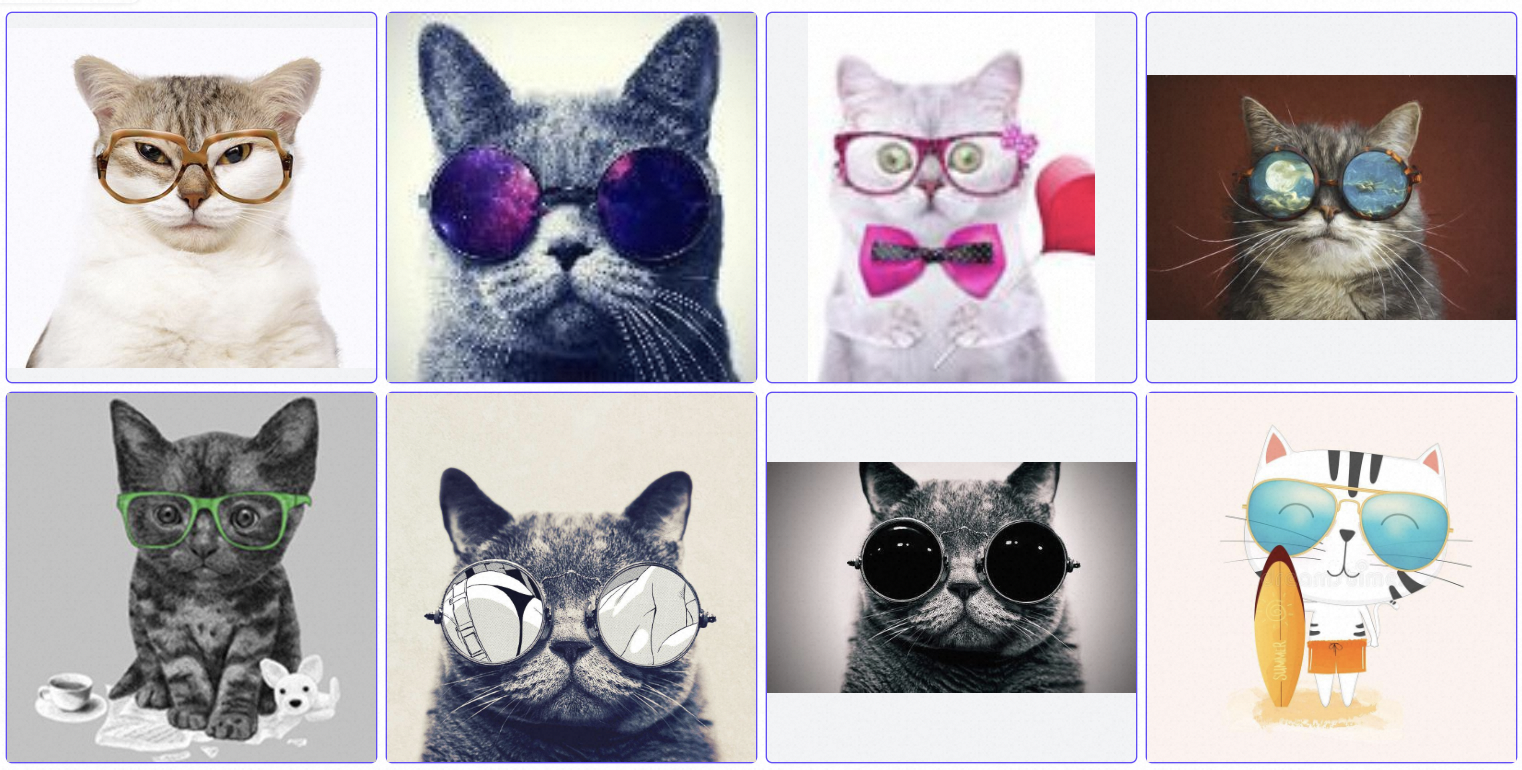
\includegraphics[width=1.0\linewidth]{pics/cat.png}
    \caption{Retrieval results of the query ``a cat with glasses'' in Chinese.}
    \label{fig:demo_cat}
\end{figure*}

\begin{figure*}[h] 
    \centering
    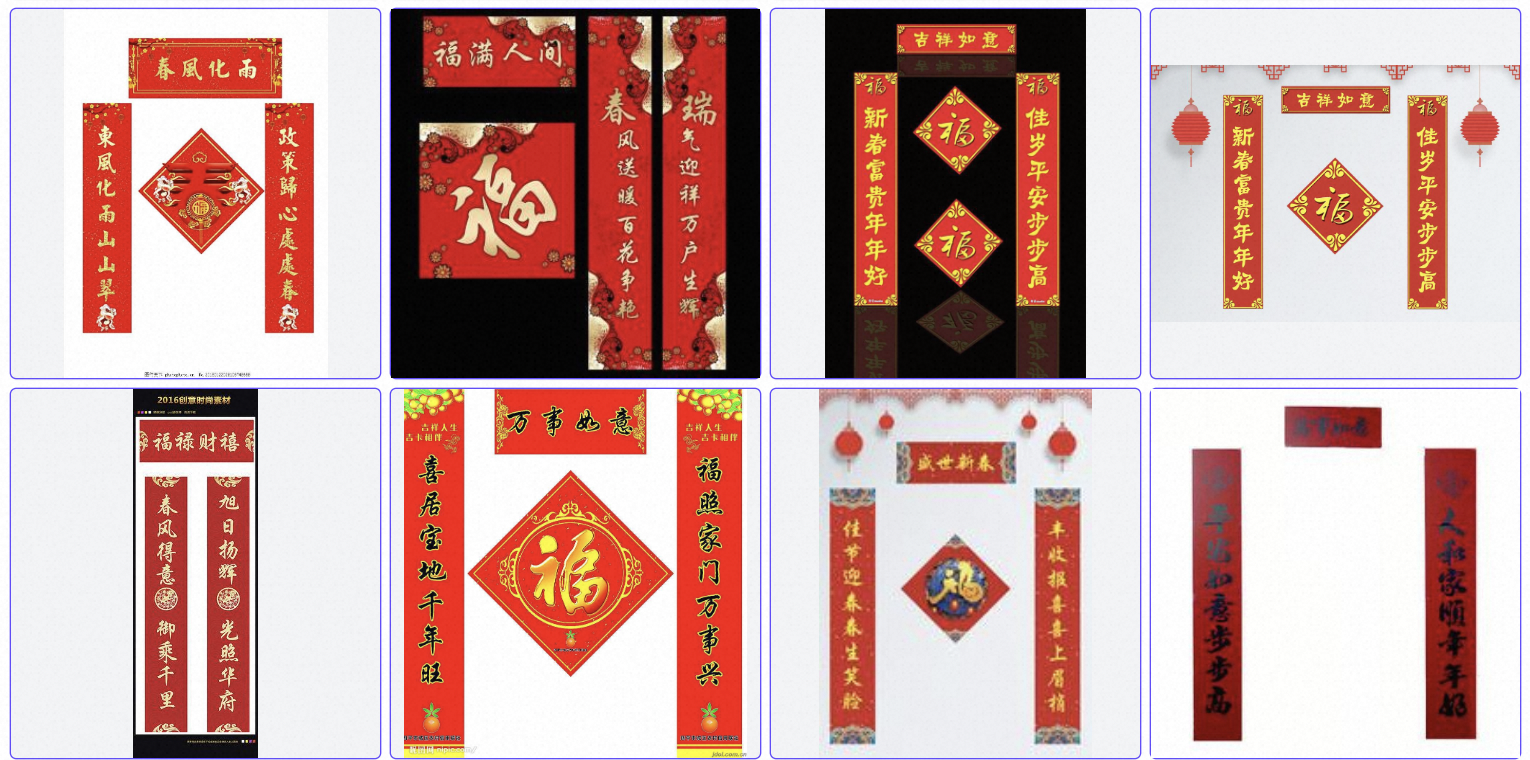
\includegraphics[width=1.0\linewidth]{pics/couplet.png}
    \caption{Retrieval results of the query ``Spring Festival couplet'' in Chinese.}
    \label{fig:demo_couplet}
\end{figure*}